\chapter{中央データベースとローカルデータベースの同期}

この章では中央データベースとローカルデータベースのデータ同期機能に関しての調査と各ツールにおける改善策の考案、処理時間測定を行った。
詳細について以下で説明する。

\section{サーバーの設置場所による処理時間の違い}
4章で述べたように、中央データベースはチェコに設置されている。
そのため試験結果のアップロードに関して、各組み立て機関から接続しデータ送信する処理時間は、機関の場所に大きく依存すると考えられる。
世界的にデータ同期ツールが不自由なく動くことに向けた開発、改善に役立てることを目的として、データベース間の情報通信にかかる処理時間を、以下の3つの場所に置かれているサーバーを用いて測定した。
組み立て機関及びローカルデータベースの設置場所はヨーロッパ、アメリカ、日本の3つの地域に分布している(付録\ref{cap:appA})。
それぞれにおける代表機関として以下の3つに設置されたサーバーを用いて調査を行った。

\begin{itemize}
  \item 日本、高エネルギー加速器研究所(KEK) 
  \item アメリカ、バークレー研究所(LBL)
  \item スイス、欧州原子核研究機構(CERN)
\end{itemize}

各サーバーの性能を表\ref{server_spec}に示す。また各サーバーが置かれている場所の位置関係を図\ref{server_geometry}に示す。

\begin{table}[tbp]
\caption[各ローカルデータベースサーバーの性能一覧]{各ローカルデータベースサーバーの性能一覧。今回の調査に利用したサーバーの性能を示す。KEK(日本)、LBL(アメリカ)、CERN(スイス)に設置されたサーバーを用いた。}
\label{server_spec}
\scalebox{0.9}{
  \small
  \begin{tabular}{|l|llll|l|l|} \hline
    設置機関 & CPU & & & & Memory & Disk \\
     & Type & Core & Thread & Clock speed[GHz]& [GB] & [GB] \\ \hline 
    KEK(日本) & Intel(R) Core(TM) i7-9700K & 8 & 16 & 3.6 & 32.66 & 1800 + 1800\\
    LBL(アメリカ) & Intel(R) Core(TM) i7-8700 & 6 & 12 & 3.7 & 32.63 & 233\\
    CERN(スイス) & Intel(R) Core(TM) i7-4790 & 4 & 8 & 3.6 & 32.69 & 238.5 + 3700 + 3700\\ \hline
  \end{tabular}
}
\end{table}

\begin{figure}[bpt]\centering
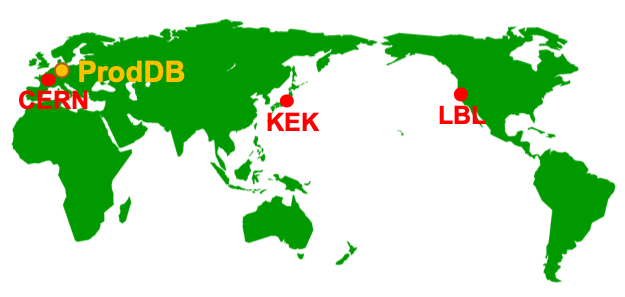
\includegraphics[width=10cm]{./server_geometry.png}
\caption[各サーバーの設置場所]{各サーバーの設置場所。赤点で示しているのがそれぞれローカルデータベースサーバーの設置位置であり、オレンジで示しているのが中央データベースである。距離としてはCERNが一番近く、LBL、KEKの順番となっている。}
\label{server_geometry}
\end{figure}

これらのサーバーは実際に生産の際に使用するものと同程度の性能を持ち、サーバーが置かれているネットワーク環境も生産時と同じであると仮定している。

\subsection{データ同期ツールに使用するAPI}
中央データベースのデータ取得には、開発されたAPIをいくつか使用している。
ローカルデータベースとのデータ同期ツールの中で主に使用しているAPIを表\ref{pd_API}に示す。

\begin{table}[tbp]
  \begin{center}
  \caption[データ同期ツールの中で使用する中央データベースの主なAPI一覧]{データ同期ツールの中で使用する中央データベースの主なAPI一覧。データ同期ツールにおいて、中央データベースの情報取得には提供されているいくつかのAPIを用いており代表的なものをいかに示す。このAPIをPythonを用いて実行することで、情報取得や試験結果のアップロードをすることができる。}
  \label{pd_API}
  \scalebox{0.7}{
    \begin{tabular}{|lll|} \hline
      関数名 & 処理の内容 & 本ツールでの使用用途\\ \hline
      getComponent            & 
      登録した部品情報の取得 & 主にダウンロード時におけるモジュールやチップの情報取得に用いる。\\
      listComponents            & 
      登録した部品情報一覧の取得 & 主にダウンロード時におけるモジュール情報一覧取得に用いる。\\
      uploadTestRunResults    & 
      テスト結果生成 & 読み出し試験結果生成の際に用いる。 \\
      createTestRunAttachment & 
      あるテスト結果に対するバイナリファイルの添付 & 読み出し試験結果生成後にファイルを添付する際に用いる。\\ \hline
    \end{tabular}
  }
  \end{center}
\end{table}

\subsection{API使用にかかる時間}
上述したAPI使用時の処理時間を各サーバーで測定した。
以下の3つの測定を行なった。
\begin{itemize}
  \item getComponentを用いた、登録モジュール情報1つの取得時間測定.
  \item createTestRunAttachmentを用いて、ある試験結果ページに1Byteのデータファイルを添付する時間測定.
  \item createTestRunAttachmentを用いて、ある試験結果ページに容量の異なるデータファイルを添付、容量に対する時間依存性を測定.
\end{itemize}

最初の2項目に関して、まとめたものを表\ref{use_prodDB_API}に示す。
ファイル容量と処理時間の関係を図\ref{datasize_vs_time}に示す
ここで、どの場合においてもKEKにおける処理時間が最も長いことがわかる。
そのため、KEKにおける処理時間を測定し、ツールの開発、改善について考えることとした。

\begin{table}[tbp]
  \caption[中央データベースAPI実行時の処理時間測定結果。]{中央データベースAPI実行時の処理時間測定結果。左の結果は表\ref{pd_API}における"getComponent"を用いてモジュール1つの情報を取得するのにかかった時間、右は"createTestRunAttachment"を用いて1Byteのファイル送信にかかった時間である。どのサーバーにおいても0.3秒以上の処理時間がかかっていることがわかり、データベースへの接続、情報取得にかかる時間が読み取れる。3つのサーバーを比べると、どちらの場合もKEKサーバーでの処理時間が一番大きいことが分かる。}
  \label{use_prodDB_API}
  \begin{minipage}[t]{.45\textwidth}
  \begin{center}
    \begin{tabular}{|ll|} \hline
      サーバー & 処理時間[秒] \\ \hline
      KEK & 0.47 $\pm$ 0.01 \\ 
      LBL & 0.37 $\pm$ 0.02 \\ 
      CERN & 0.28 $\pm$ 0.01 \\ \hline 
    \end{tabular}
  \end{center}
  \end{minipage}
  \hfill 
  \begin{minipage}[t]{.45\textwidth}
  \begin{center}
    \begin{tabular}{|ll|} \hline
      サーバー & 処理時間[秒] \\ \hline
      KEK & 0.83 $\pm$ 0.01 \\ 
      LBL & 0.34 $\pm$ 0.03 \\ 
      CERN & 0.48 $\pm$ 0.03 \\ \hline 
    \end{tabular}
  \end{center}
  \end{minipage}
\end{table}

\begin{figure}[bpt]\centering
  \begin{center}
    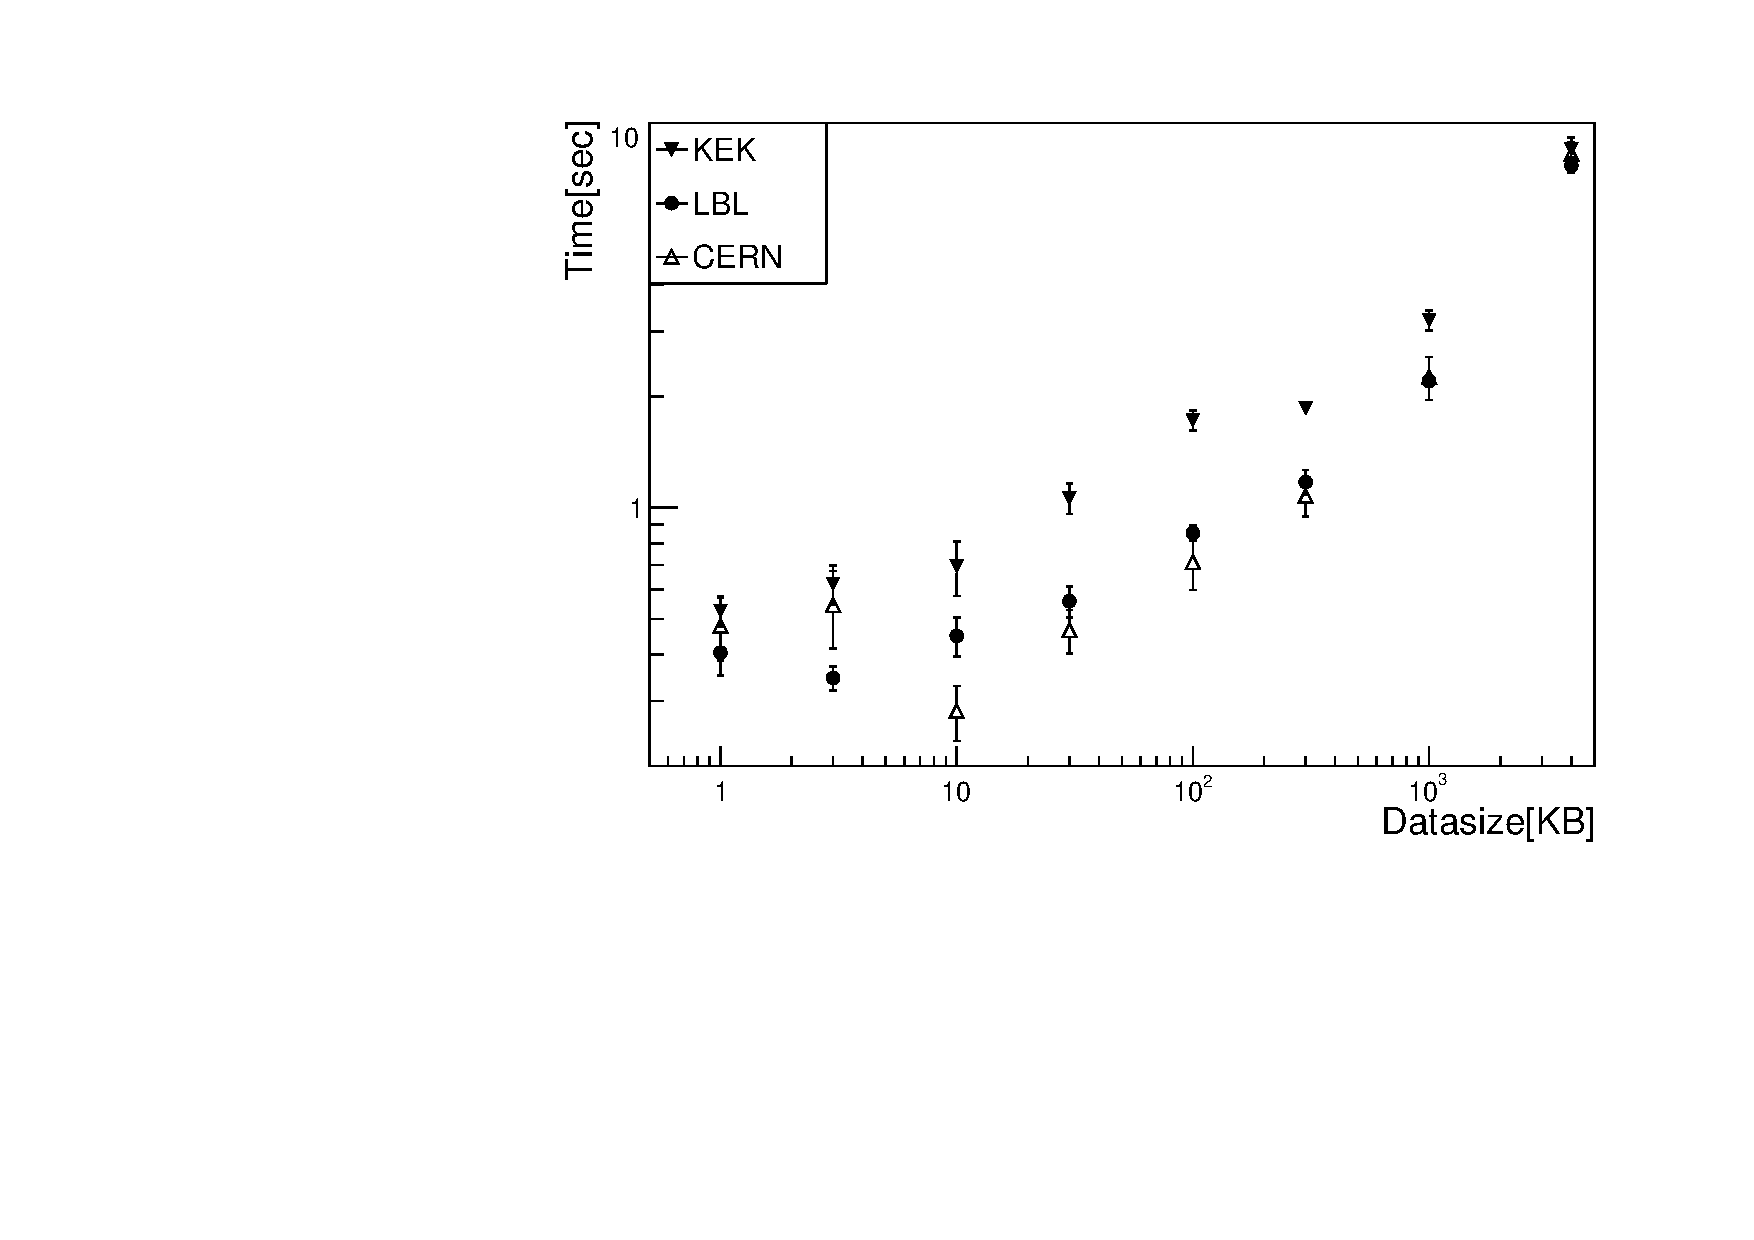
\includegraphics[width=8cm,angle=270]{./datasize_vs_time_new.pdf}
  \caption["createTestRunAttachment"を用いた添付処理におけるファイル容量と処理時間の関係]{"createTestRunAttachment"を用いた添付処理におけるファイル容量と処理時間の関係。それぞれのサーバーで1、3、10、30、100、300KB、1、4MBのファイル送信にかかる時間を測定した。どの点においてもKEKサーバーが最も処理時間を要していることが分かる。またこのグラフについての詳しい考察を付録\ref{chap:data_time_detail}に記す。}
  \label{datasize_vs_time}
  \end{center}
\end{figure}

%%%%%%%%%%%%%%%%%%%%%%%%%%%%%%%%%%%%%%%%%%%%%%%%%%%%%%%%%%
%%%%%%%%%%%%%%%%%%%%%%%%%%%%%%%%%%%%%%%%%%%%%%%%%%%%%%%%%%
%%%%%%%%%%%%%%%%%%%%%%%%%%%%%%%%%%%%%%%%%%%%%%%%%%%%%%%%%%

\clearpage
\section{モジュール情報のダウンロード}
\subsection{ダウンロードする情報と構造}
中央データベースから、モジュール及びFEチップの情報をダウンロードする機能を開発、実装した。
ダウンロードする情報の詳細について表\ref{download_information}に示す。

\begin{table}[tbp]
\begin{center}
\caption[ダウンロード機能を用いて保存する情報一覧。]{ダウンロード機能を用いて保存する情報一覧。ダウンロード機能を用いて中央データベースからローカルデータベースに保存する情報の一覧を示している。保存の際にはモジュール、FEチップにそれぞれ分かれたドキュメントに保存される。}
\label{download_information}
  \small
  \begin{tabular}{|ll|} \hline
    部品 & 情報 \\ \hline
    モジュール & シリアルナンバー \\ 
     & 搭載FEチップの種類  \\ 
     & 登録機関  \\ 
     & 搭載FEチップの枚数  \\ \hline 
    FEチップ & シリアルナンバー \\
     & FEチップID(モジュール上の位置を表す情報) \\  
     & 登録機関 \\ \hline 
  \end{tabular}
\end{center}
\end{table}

ダウンロードされたモジュール、FEチップのドキュメントの例をリスト\ref{download_module_document}、\ref{download_fechip_document}に示す。
\begin{lstlisting}[basicstyle=\scriptsize,caption=ダウンロードしたモジュール情報のドキュメントの例。ドキュメントが表\ref{download_information}の情報を持つことが分かる。,label=download_module_document]
{
	"_id" : ObjectId("5fa79114e615fa000a1a5976"),
	"name" : "20UPGR00000001",
	"chipType" : "RD53A",
	"serialNumber" : "20UPGR00000001",
	"chipId" : -1,
	"componentType" : "module",
	"address" : "5fd597fdf7339bbf26b87fb2",
	"children" : 1,
	"sys" : {
		"mts" : ISODate("2020-12-13T04:26:37.989Z"),
		"cts" : ISODate("2020-12-13T04:26:37.989Z"),
		"rev" : 0
	},
	"dbVersion" : 1.01,
	"user_id" : -1,
	"proDB" : true
}
\end{lstlisting}
\begin{lstlisting}[basicstyle=\scriptsize,caption=ダウンロードしたFEチップ情報のドキュメントの例。ドキュメントが表\ref{download_information}の情報を持つことが分かる。,label=download_fechip_document]
{
	"_id" : ObjectId("5fa79560e615fa000a1a5a16"),
	"name" : "20UPGFC9999999",
	"chipType" : "RD53A",
	"serialNumber" : "20UPGFC9999999",
	"chipId" : 0,
	"componentType" : "front-end_chip",
	"address" : "5fd597fdf7339bbf26b87fb2",
	"children" : -1,
	"sys" : {
		"mts" : ISODate("2020-12-13T04:26:37.984Z"),
		"cts" : ISODate("2020-12-13T04:26:37.984Z"),
		"rev" : 0
	},
	"dbVersion" : 1.01,
	"user_id" : -1,
	"proDB" : true
}
\end{lstlisting}

\subsection{処理の流れ}

ダウンロード機能における処理の流れのイメージを図\ref{download_algorithm}に示す。

\begin{figure}[bpt]\centering
  \begin{center}
  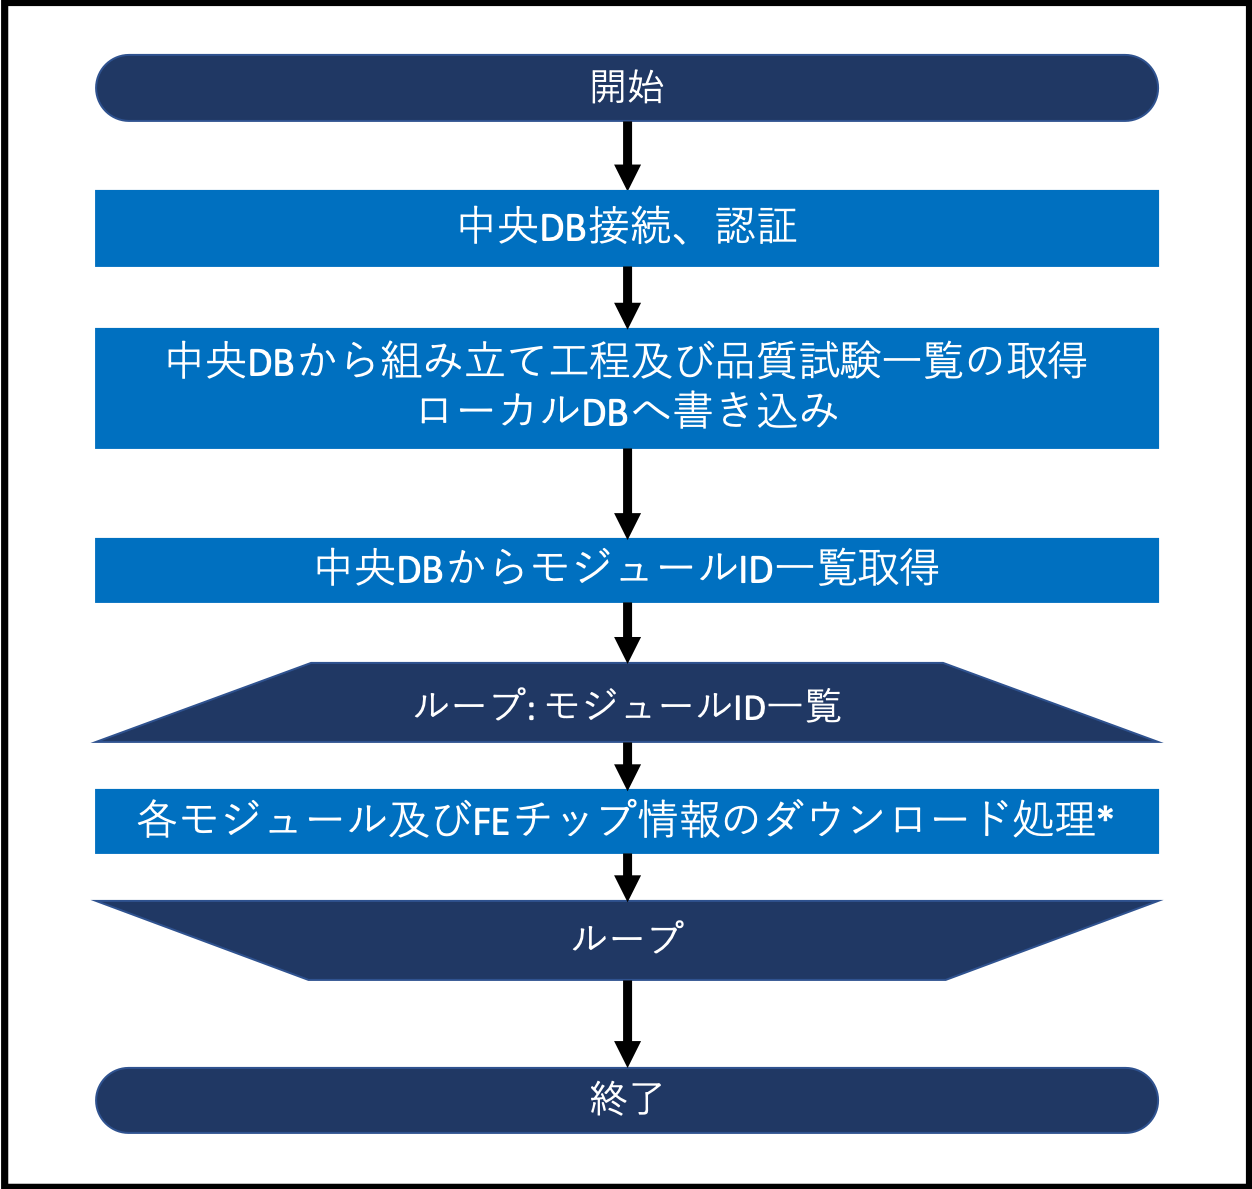
\includegraphics[width=11cm]{./download_tool_flow_whole.png}
  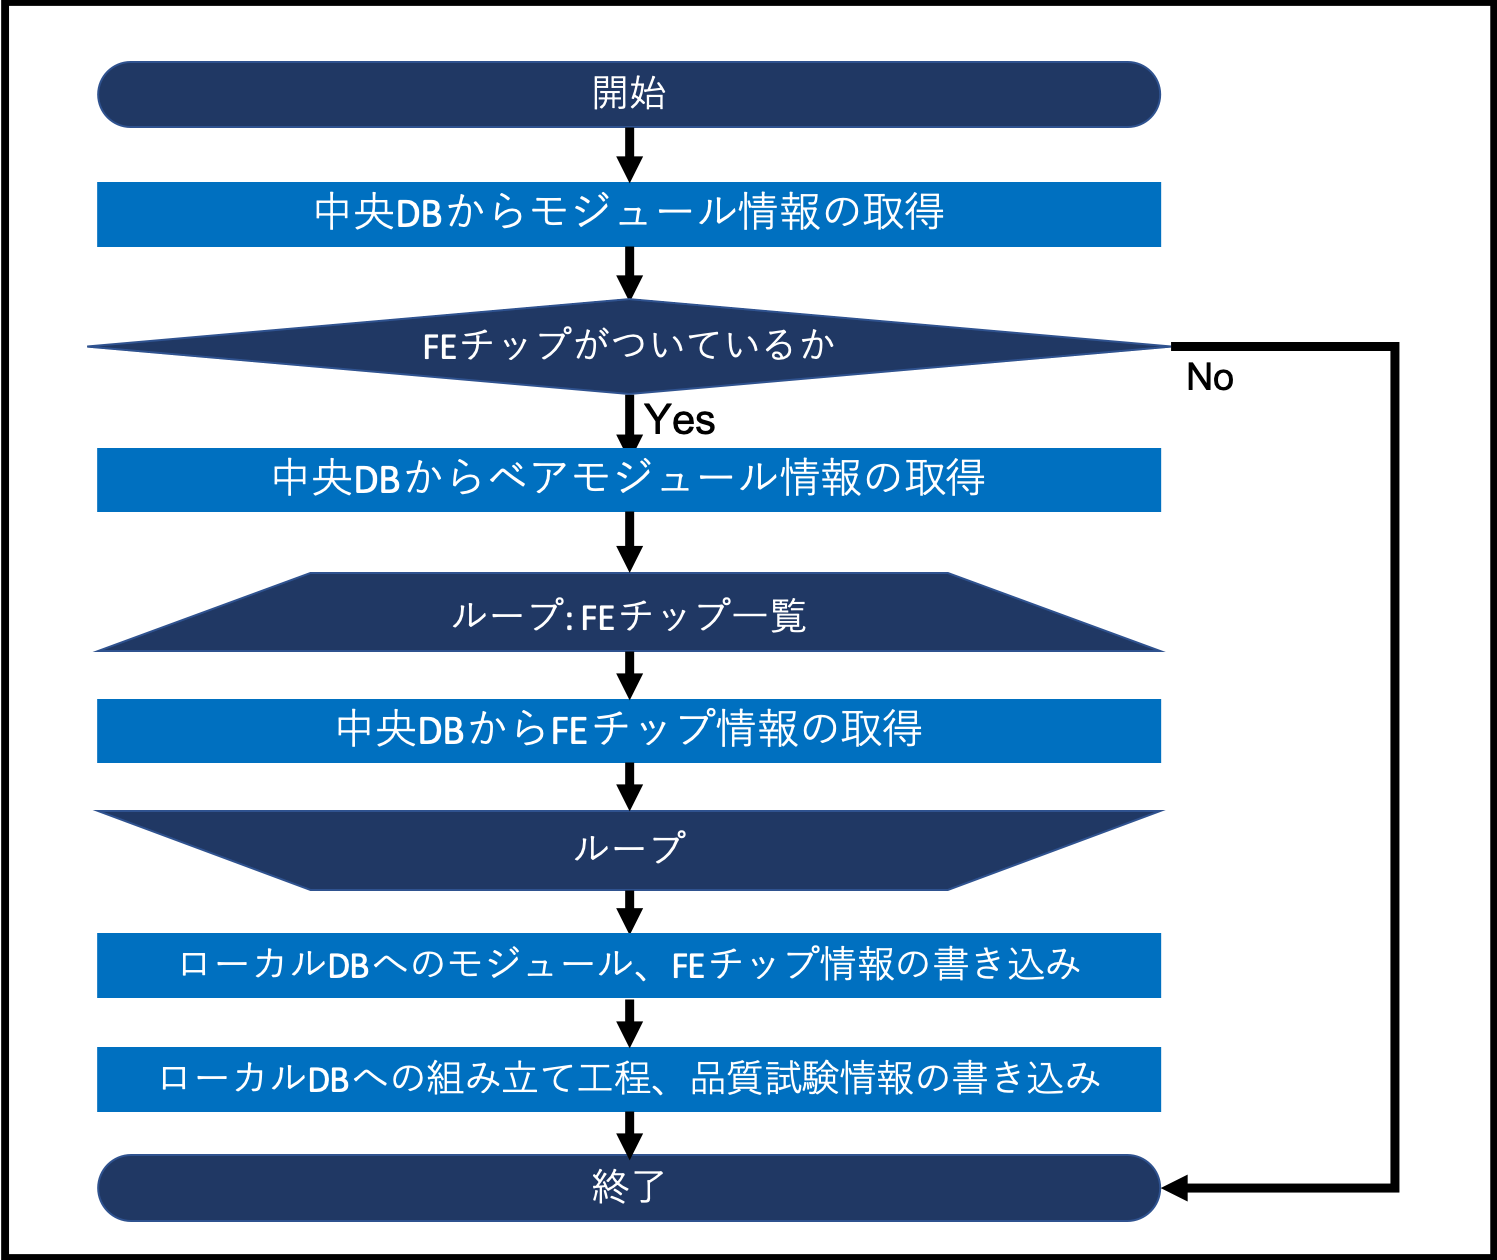
\includegraphics[width=11cm]{./download_tool_flow_detail.png}
  \caption[ダウンロード処理における流れのイメージ図]{ダウンロード処理における流れのイメージ図。上図が処理全体の流れを表すものであり、下図は各モジュール情報のダウンロードにおける処理の流れを示している。上図中のループ構造の1処理が下図に対応している。流れの中で複数回中央データベースに接続し、モジュールやFEチップの情報取得をしていることが分かる。}
  \label{download_algorithm}
  \end{center}
\end{figure}

\subsection{機能確認}
KEKで組み立てられた6台のQuadモジュールを中央データベースに登録し、ダウンロードを行った。
登録したモジュールを表\ref{registered_kek_module}、ダウンロードをしてアプリケーションで確認した様子を図\ref{registered_kek_module_viewer}に示す。

\begin{figure}[bpt]\centering
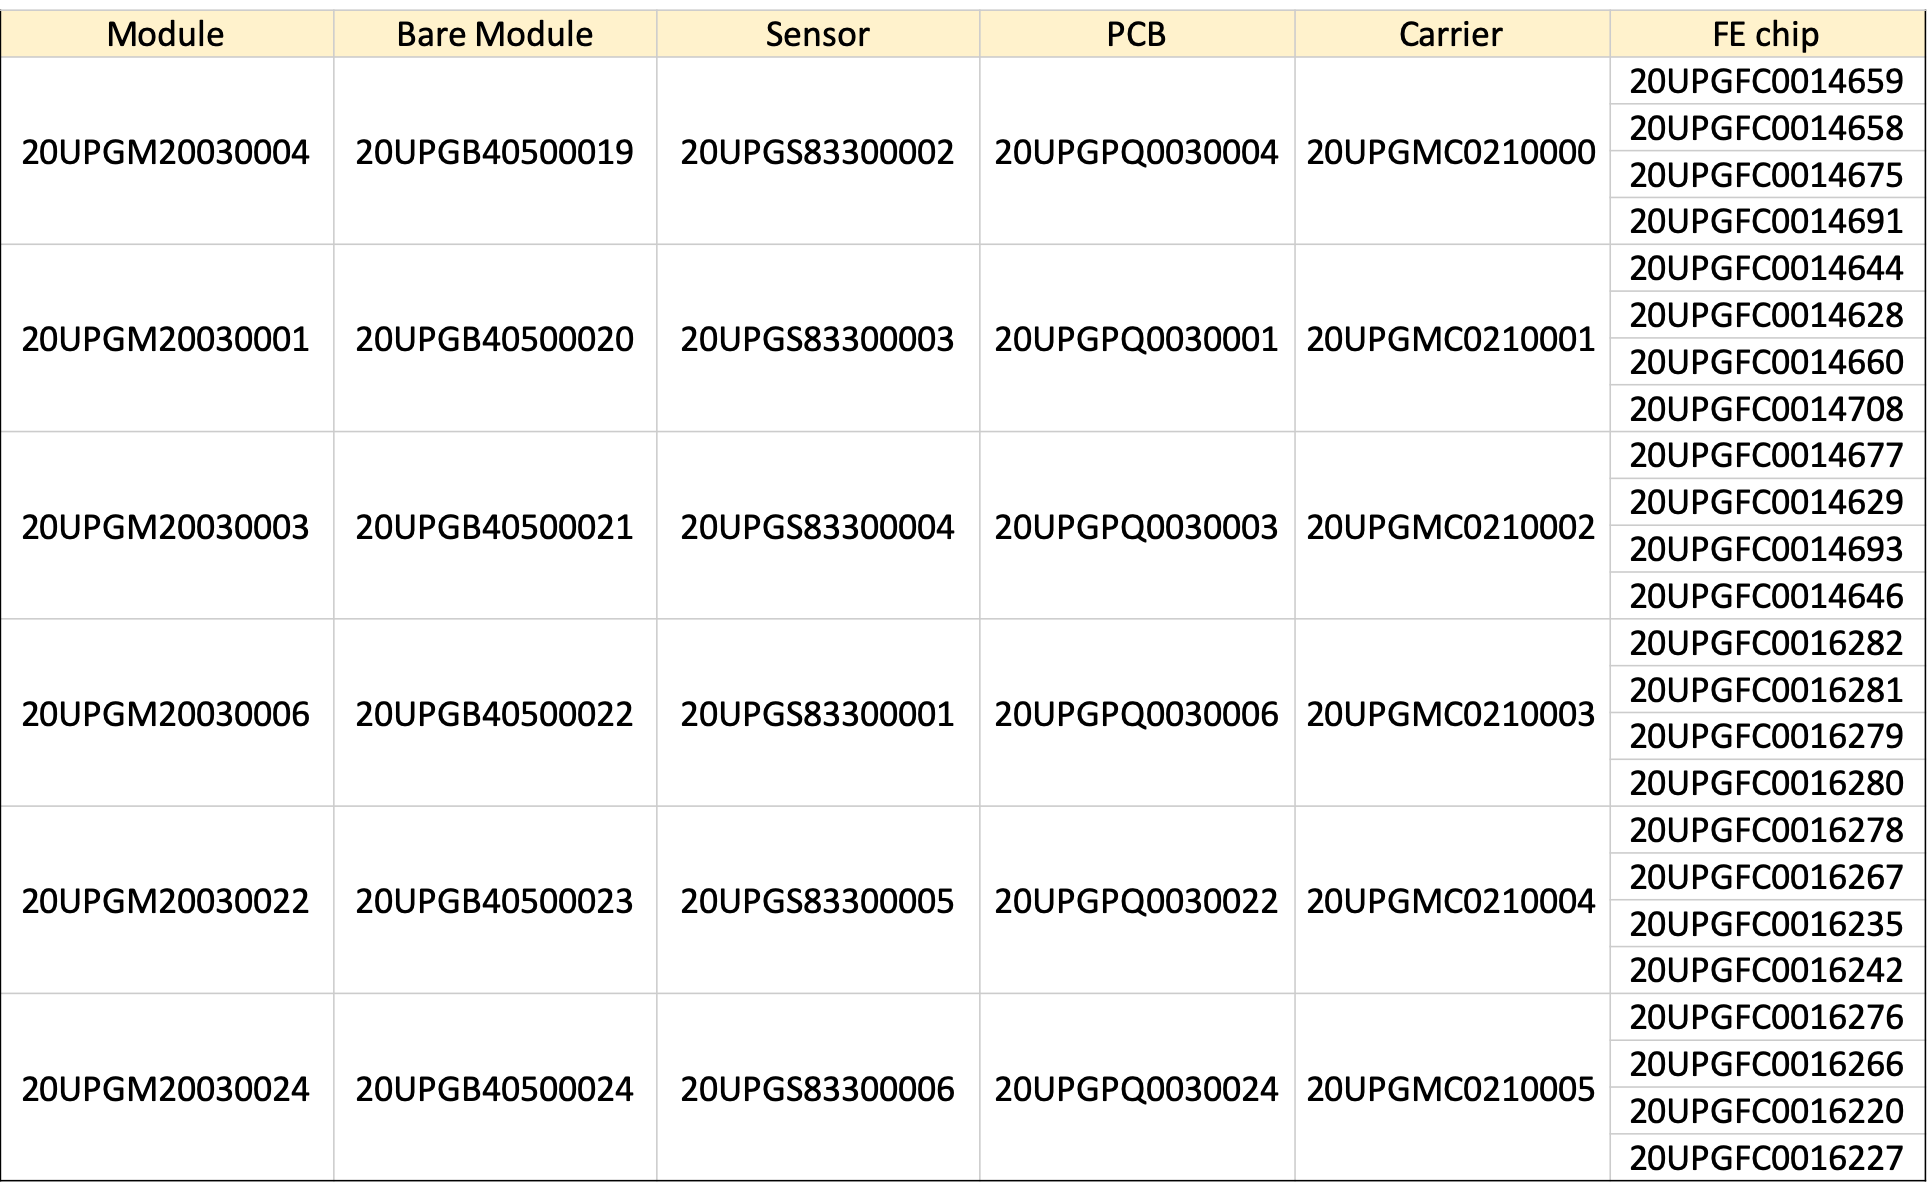
\includegraphics[width=12cm]{./registered_kek_module.png}
\caption[登録したQuadモジュールと構成部品のシリアルナンバー一覧。]{登録したQuadモジュールとその構成部品のシリアルナンバー一覧。左から、登録したモジュール、搭載されているベアモジュール、シリコンセンサー、PCB、モジュールキャリア、FEチップの中央データベース内でのシリアルナンバーを示している。Quadモジュールであるため、FEチップをそれぞれ4つ搭載している。}
\label{registered_kek_module}
\end{figure}

\begin{figure}[bpt]\centering
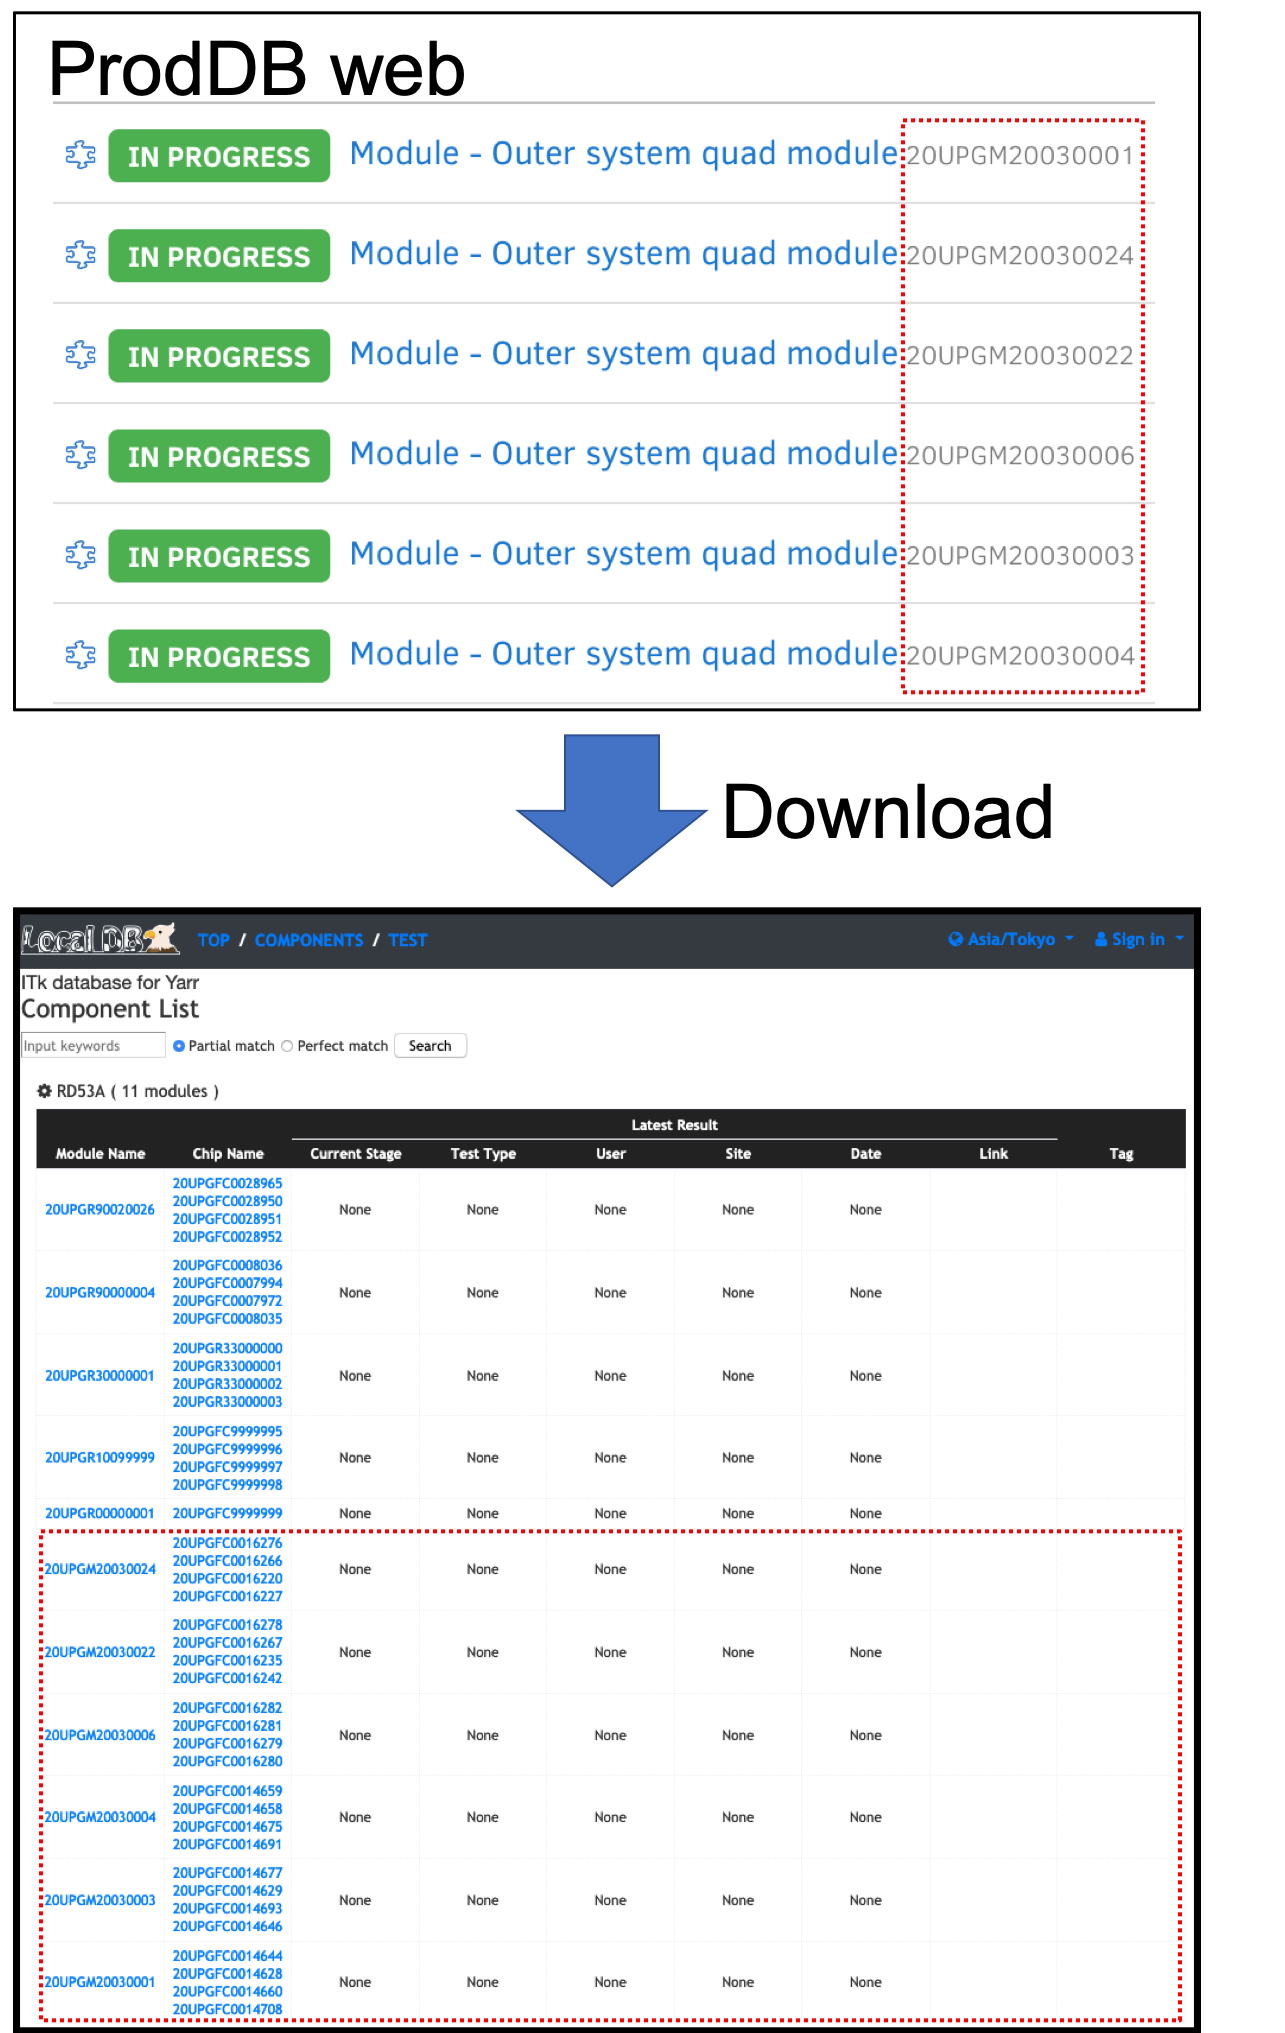
\includegraphics[width=13cm]{./registerd_kek_module_viewer.png}
\caption[登録したQuadモジュールのダウンロードの様子]{登録したQuadモジュールのダウンロードの様子。上図が中央データベースのウェブページを表しており、下図がローカルデータベースのものである。上図で登録したモジュール一覧を確認でき、赤枠で囲っているところでシリアルナンバーを見ることができる。ダウンロード実行後は下図のようにローカルデータベースで対応するモジュールを確認することができる。ローカルデータベースではモジュール情報に加えてFEチップの情報も取得するため、下図の表ではこれらのシリアルナンバーも確認できる。}
\label{registered_kek_module_viewer}
\end{figure}

\subsection{処理時間測定}
ダウンロードの処理時間を測定した。
これについてまとめたものを表\ref{download_measurement}に示す。
Quadモジュール1つに対して平均して4.0 $\pm$ 0.4秒の処理時間がかかっている。

\begin{table}[tbp]
\begin{center}
\caption[登録したモジュールのダウンロード処理時間測定結果]{登録したモジュールのダウンロード処理時間測定結果。登録したそれぞれのモジュールについてダウンロードにかかる時間を測定した。表より1つあたり平均4秒の時間がかかっていることが分かる。}
\label{download_measurement}
  \begin{tabular}{|ll|} \hline
    モジュール & 処理時間 \\ \hline
    20UPGM20030004 &  3.8 \\ 
    20UPGM20030001 &  3.7 \\ 
    20UPGM20030003 &  5.9 \\ 
    20UPGM20030006 &  3.6 \\ 
    20UPGM20030022 &  3.8 \\ 
    20UPGM20030024 &  3.3 \\ \hline 
    平均           &  4.0 $\pm$ 0.4 \\\hline
  \end{tabular}
\end{center}
\end{table}

\subsection{処理時間詳細}
ダウンロード処理時間の改善に向けて、処理時間の詳細について以下の測定した。
\begin{enumerate}
  \item 中央データベースからモジュール情報の取得.
  \item データベースでのFEチップ確認処理.
  \item 中央データベースからベアモジュール情報の取得.
  \item 中央データベースからFEチップ情報の取得(4枚分).
  \item ローカルデータベースへの情報の書き込み(モジュール、FEチップ、品質試験情報).
\end{enumerate}

情報取得のイメージを表\ref{download_process_image}に示す。
このようにQuadモジュールの場合、ダウンロードの流れの中で合計して7回、データベースAPIを用いて情報取得を行う。
\begin{figure}[bpt]\centering
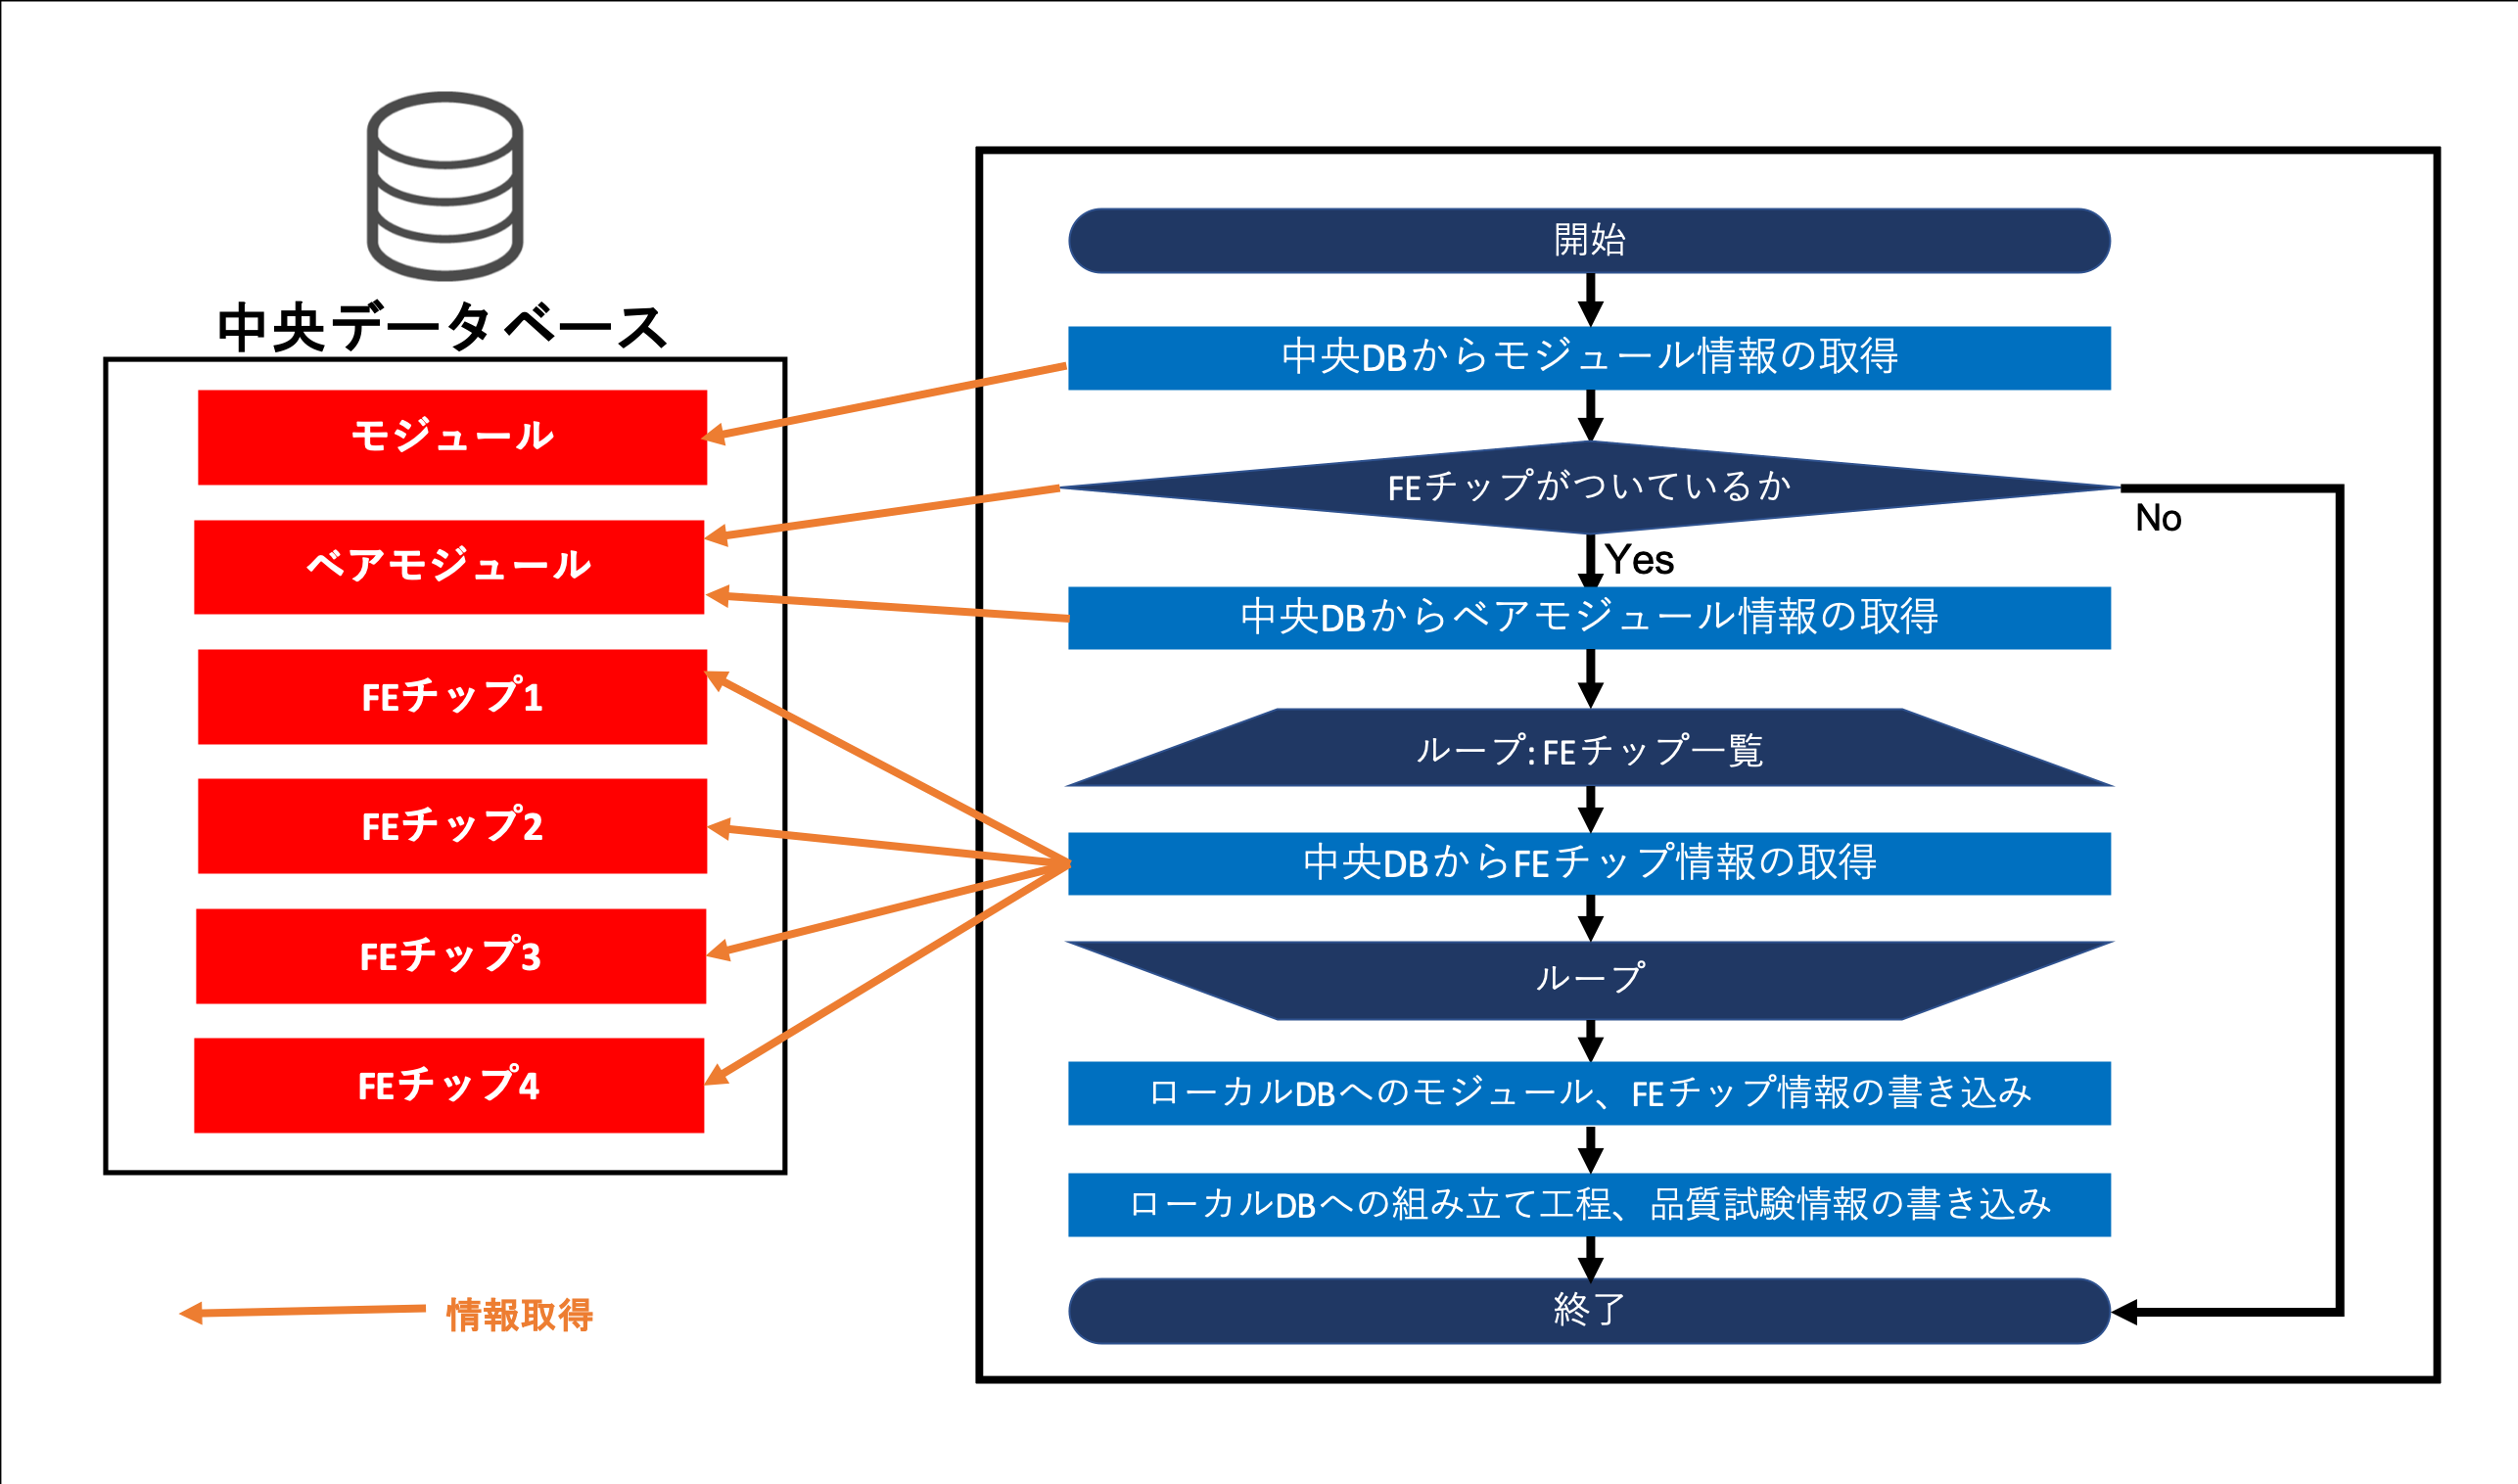
\includegraphics[width=15cm]{./download_process_image.png}
\caption[モジュール及び構成部品情報取得のイメージ図]{モジュール及び構成部品情報取得のイメージ。図のように処理の流れの中で合計7回中央データベースに接続し、モジュール、ベアモジュール、 FEチップの情報取得を行っている。}
\label{download_process_image}
\end{figure}

結果を表\ref{download_process_details}に示す。
\begin{table}[tbp]
\begin{center}
\caption[ダウンロード機能における詳細処理にかかる時間測定]{ダウンロード機能における詳細処理にかかる時間測定。図\ref{download_process_image}より、中央データベースに接続、情報取得を合計して7回行っており、それが処理1から4に対応する。どの処理においても0.5秒程度の時間がかかっていることが分かる。処理5はローカルデータベースへの書き込み処理であるが、他の処理に比べて十分に小さいことが分かる。}
\label{download_process_details}
  \begin{tabular}{|ll|} \hline
    処理 & 時間 \\ \hline
    1 &  0.60 $\pm$ 0.07 \\ 
    2 &  0.55 $\pm$ 0.07 \\ 
    3 &  0.61 $\pm$ 0.04 \\ 
    4 &  0.46 $\pm$ 0.04 \\ 
      &  0.71 $\pm$ 0.19 \\ 
      &  0.51 $\pm$ 0.04 \\ 
      &  0.57 $\pm$ 0.12 \\ 
    5 &  0.0025 $\pm$ 0.0011 \\ 
    合計 & 4.0 $\pm$ 0.1 \\ \hline
  \end{tabular}
  \begin{tablenotes}
    \item[1] 1. 中央データベースからモジュール情報の取得.
    \item[2] 2. データベースでのFEチップ確認処理.
    \item[3] 3. 中央データベースからベアモジュール情報の取得.
    \item[4] 4. 中央データベースからFEチップ情報の取得(4枚分).
    \item[5] 5. ローカルデータベースへの情報の書き込み(モジュール、FEチップ、品質試験情報).
  \end{tablenotes}
\end{center}
\end{table}

この結果より、各構成部品情報の取得(モジュール、ベアモジュール、FEチップ)の取得にそれぞれ均等に処理時間がかかっていることがわかった。

\subsection{生産時における見積もり}
現在ダウンロード機能のオプションとして、以下の2つを実装している。
\begin{enumerate}
  \item モジュール1つをダウンロードする機能.
  \item 登録されている全てのモジュールの一括ダウンロード機能.
\end{enumerate}

オプション1の見積もり値は、表\ref{download_measurement}の平均値として$4.0\pm0.4$[sec]となる。
オプション2の見積もり値は、生産時には最大で10,000台のモジュールが中央データベースに登録されることから、以下のようになる。
\bbb
(4.0 \pm 0.4)[\rm{sec}] \times 10,000 = 11 \pm 1 [{\rm hour}]
\eee

各機関で各モジュールの組み立てを始める際に、中央データベースへのモジュール登録及びローカルデータベースへのダウンロードを行うことを想定している。
これは1つずつ行うため、このような場合はオプション1を用いる。

オプション2の使用例として、モジュールの組み立て工程の途中で、複数のモジュール($O(100)$程度)を機関1から機関2に輸送する場合をあげる。
機関2では機関1で登録された全てのモジュール情報をダウンロードしてくる必要があるため、このオプションを使用する。
輸送に要する時間として1日と仮定すると、この時間を利用してダウンロード処理を行う必要がある。

\subsection{改善点の考案と見積もり}

オプション2について、11時間の処理時間を要する見積もりとなっている。
より円滑な同期処理に向けて、改善方法について考える。

一括ダウンロード機能については以下の改善点が考えられる。
\begin{enumerate}
  \item モジュールの現在位置に対応したもののみのダウンロード.
  \item FEチップの登録機関を取得しない.
  \item モジュールのプロパティとして、ダウンロードに必要な情報を全て保存.
  \item データベースAPIを改良し、モジュール一覧取得の際に構成要素の情報を取得できるようにする.
\end{enumerate}

これらについて詳細と処理時間の見積もりを以下で行う。

\subsubsection{改善案1: モジュールの現在位置に対応したもののみのダウンロード}
上述した機関が途中で変更となるような組み立ての流れにおいて、全てのモジュールIDをダウンロードする必要はない。
中央データベースにはモジュールの現在位置情報を保持しているため、機能実行者と位置が同じもののみをダウンロードするアルゴリズムにすれば処理時間を改善できる。
見積もりとしては、ダウンロード対象となるモジュール数を$n$とすると、以下のようになる。
\bbb
( 11 \pm 1 ) \times \frac{n}{10000} [{\rm hour}]
\eee

\subsubsection{改善案2: FEチップの登録機関を取得しない}
表\ref{download_process_image}よりダウンロードの際に、FEチップの情報取得を行っている。
これはFEチップ登録機関の情報を取得しローカルデータベースに保存するためであるが、登録機関の情報は組み立て現場で扱う作業としては、必要な情報ではない。
そのため、現段階ではFEチップのデータ取得処理は割愛することができる。
これにかかる処理時間は表\ref{download_process_details}より、合計して$2.3\pm0.2$[sec]となるため、その場合オプション2の処理時間の見積もりは、
以下のようになる。
\bbb
\{(4.0 \pm 0.4) - (2.3 \pm 0.2)\}[\rm{sec}] \times 10,000 =4.9 \pm 0.8 [{\rm hour}]
\eee
この改善策のデメリットとしては、FEチップの情報取得処理を省くとローカルデータベースで扱いたい情報が将来的にできた場合に保存できないことである。
例えば各FEチップの最適動作電圧のようにモジュール読み出しに対して有益な情報は保存し、迅速に確認したいという方針になる可能性もある。

\subsubsection{改善案3: モジュールのプロパティとして、ダウンロードに必要な情報を全て保存}
モジュールのプロパティとして、FEチップの名前等のダウンロードに必要な情報を書いておくと、表\ref{pd_API}におけるlistComponentsによるモジュール一覧取得でその情報を参照することができる。
こうすることで、表\ref{download_process_image}において、ベアモジュールやFEチップの情報取得を省くことができる。
この場合処理時間は、合計して$2.9\pm0.2$[sec]となるため、その場合オプション2の処理時間の見積もりは、
\bbb
\{(4.0 \pm 0.4) - (2.9 \pm 0.2)\}[\rm{sec}] \times 10,000 =3.1 \pm 0.8 [{\rm hour}] 
\eee

これのデメリットは、データベースの中でデータが冗長になってしまうことである。
FEチップの名前情報がモジュールのプロパティにも保存されていると、データベース内部で冗長性を持ってしまい、編集が加えられた場合などこれを管理するのが難しくなる。

\subsubsection{改善案4:データベースAPIを改良し、モジュール一覧取得の際に構成要素の情報を取得できるようにする}
現在、表\ref{pd_API}のlistComponentsを用いた時にはモジュール一覧の情報は取得できるが、各モジュールに対して構成要素は取得できない。
そのため表\ref{download_process_image}のようにモジュールごとに中央データベースに接続し、部品情報を取得している。
ダウンロードに必要な情報をlistComponentsで一括で取得できるような仕様にAPIの変更を行えば、中央データベースへの接続は一回ですみ、処理時間を削減できると考えられる。
この場合、中央データベースの内部構造を知り、一括で取得しデータ送信をする場合にどれだけの時間を要するかを見積もり、今の場合と比較する必要がある。\\


現段階では組み立ての試験段階であり、現場で必要な情報、世界各地での組み立て工程の流れ等を検討している段階である。
ここで述べたような改善策を組み合わせ、変更を加えていく必要がある。
また中央データベースとの同期におけるネットワーク速度は地理的な距離により異なるため、この点も考慮に入れる必要がある。
今回のは日本での測定であるため、他の国においては処理速度は改善すると考えられる。

%%%%%%%%%%%%%%%%%%%%%%%%%%%%%%%%%%%%%%%%%%%%%%%%%%%%%%%%%%
%%%%%%%%%%%%%%%%%%%%%%%%%%%%%%%%%%%%%%%%%%%%%%%%%%%%%%%%%%
%%%%%%%%%%%%%%%%%%%%%%%%%%%%%%%%%%%%%%%%%%%%%%%%%%%%%%%%%%

\clearpage
\section{読み出し試験結果のアップロード}
4章で述べたように、読み出し試験結果について中央データベースへアップロードするツールを開発した。
以下で詳細を述べる。
\subsection{アップロードする情報とその構造}
読み出し試験結果について、中央データベースにアップロードする情報を以下に記す。
\begin{itemize}
  \item 試験日時.
  \item モジュール周りの環境温度.
  \item ピクセル解析結果.
  \item 各試験結果データファイル.
  \item 読み出し設定ファイル.
  \item その他設定ファイル(DB、ユーザ、組み立て機関等).
\end{itemize}

中央データベースにおける読み出し試験の構造に関して、YARRを用いて行った読み出し結果は全てFEチップ毎に取得、保存される。
そのため、データベースの内部でもFEチップに読み出し試験結果を紐つける構造を設け、モジュールの結果では各FEチップの結果ページのIDを持つ構造とした。イメージを図\ref{structure_for_electrical_tests}に示す。

\begin{figure}[bpt]\centering
  \begin{center}
  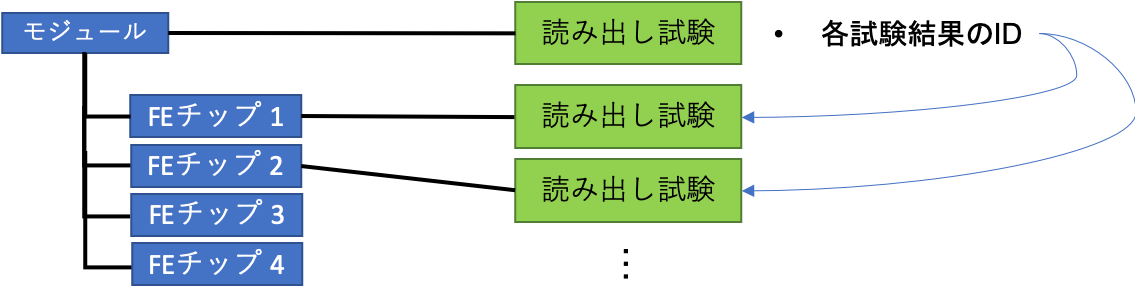
\includegraphics[width=13cm]{./structure_for_electrical_tests.png}
  \caption[中央データベースにおける読み出し試験結果の構造]{中央データベースにおける読み出し試験結果の構造。YARRの出力ファイル及びローカルデータベースのデータ構造において、読み出し試験結果は全てFEチップに紐つけられている。そのため、図のように中央データベースにおいてもこのデータ構造を保持する形でアップロードを行う。モジュールの結果は各FEチップの試験結果に対するIDを持つことで紐付けを行っている。}
  \label{structure_for_electrical_tests}
  \end{center}
\end{figure}

中央データベースにおいてモジュール、FEチップの試験結果が持つ情報を表\ref{electrical_parameters}にまとめる。
\begin{table}[tbp]
\begin{center}
\caption[中央データベースにおける読み出し試験結果に関する情報一覧]{中央データベースにおける読み出し試験結果に関する情報一覧。モジュール及びFEチップが中央データベース内で持つ試験結果の情報を示している。}
\label{electrical_parameters}
  \small
  \begin{tabular}{|l|l|l|} \hline
    部品 & 試験情報、結果 & 添付ファイル \\ \hline\hline
    モジュール &  モジュール環境温度 & \\  
               &  FEチップにつく読み出し試験結果のID & \\  \hline
    FEチップ &  ピクセル解析結果 & 試験結果データファイル\\ 
             &                   & 読み出し設定ファイル\\
             &                   & その他設定ファイル\\ \hline 
  \end{tabular}
\end{center}
\end{table}

\subsection{処理の流れ}

アップロード機能における処理の流れのイメージを図\ref{upload_algorithm}に示す。
流れの中には共通して行われる処理と、各FEチップに対して行われる処理がある。

\begin{figure}[bpt]\centering
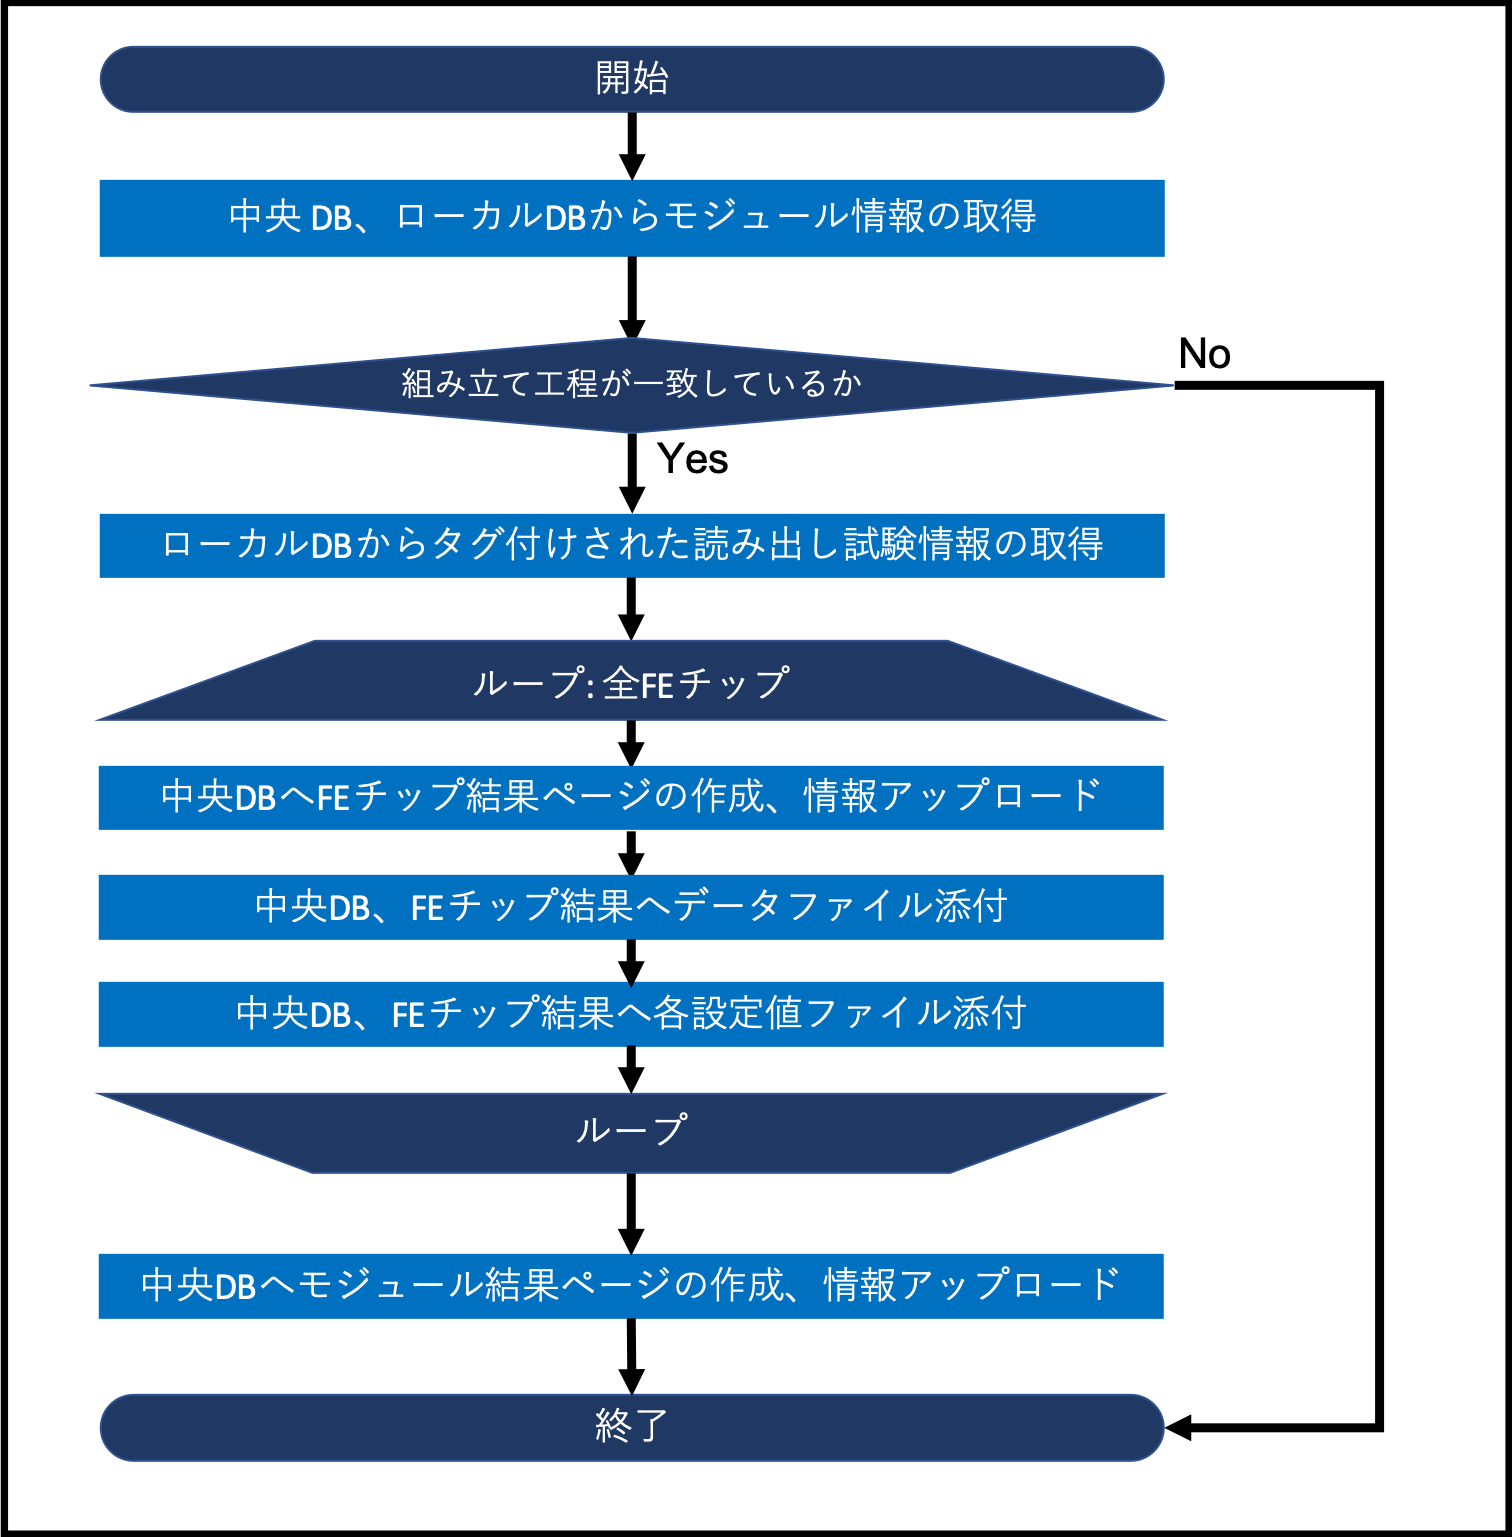
\includegraphics[width=10cm]{./upload_algorithm.png}
\caption[アップロード処理に関する流れのイメージ図]{アップロード処理に関する流れのイメージ図。流れの中にはFEチップに関するループ構造があり、ここでFEチップの結果生成、結果ファイルのアップロードを行う。最後にモジュールに対する結果生成とアップロードを行う。}
\label{upload_algorithm}
\end{figure}

\subsection{処理時間測定}
上述した処理のツールを開発し、処理時間測定を行った。
ここで行ったアップロードする試験項目は章\ref{chap:demo}で行ったデモンストレーションのものと同じで以下の項目とする。
\begin{itemize}
  \item デジタル回路読み出し
  \item アナログ回路読み出し
  \item Threshold測定
  \item ToT測定
  \item ノイズ占有率測定
\end{itemize}

これらの項目についてアップロードを行い、その処理時間を測定した。
KEKのサーバーを用いてアップロード処理を20回行い、5項目全体でかかる時間を測定した。
以下のようになった。
\bbb
  (1.3 \pm 0.0) \times 10^2 [{\rm sec}]
\eee

ここで処理流れの表\ref{upload_algorithm}より特に以下の詳細処理を抜粋し、それぞれにかかる時間を測定した。

\begin{enumerate}
  \item 中央データベース接続、認証.
  \item 中央データベース、ローカルデータベースからモジュール情報の取得.
  \item 中央データベースにFEチップ結果ページの作成。結果情報をアップロード.
  \item 2で作成した結果に対して、各データファイルを添付.
  \item 2で作成した結果に対して、各設定値ファイルを添付.
  \item 中央データベースにモジュールの結果ページの作成、結果情報をアップロード.
\end{enumerate}

結果を表\ref{upload_process_detail_result}に示す。
結果データや各設定値のファイル添付に大きく時間がかかっていることが分かった。

\begin{figure}
\begin{minipage}{0.4\textwidth}
\begin{center}
\makeatletter
\def\@captype{table}
\makeatother
\begin{tabular}{|ll|} \hline
  処理 & 時間[sec] \\ \hline
  1 & $ 14 \pm 0 $ \\  
  2 & $ 0.88 \pm 0.14 $ \\  
  3 & $ 2.2 \pm  0.1 $ \\  
  4 & $ 68 \pm 3 $ \\  
  5 & $ 44 \pm 0 $ \\ 
  6 & $ 1.8 \pm 0.1 $ \\ \hline  
\end{tabular}
\end{center}
\end{minipage}
\begin{minipage}{0.5\textwidth}
\begin{center}
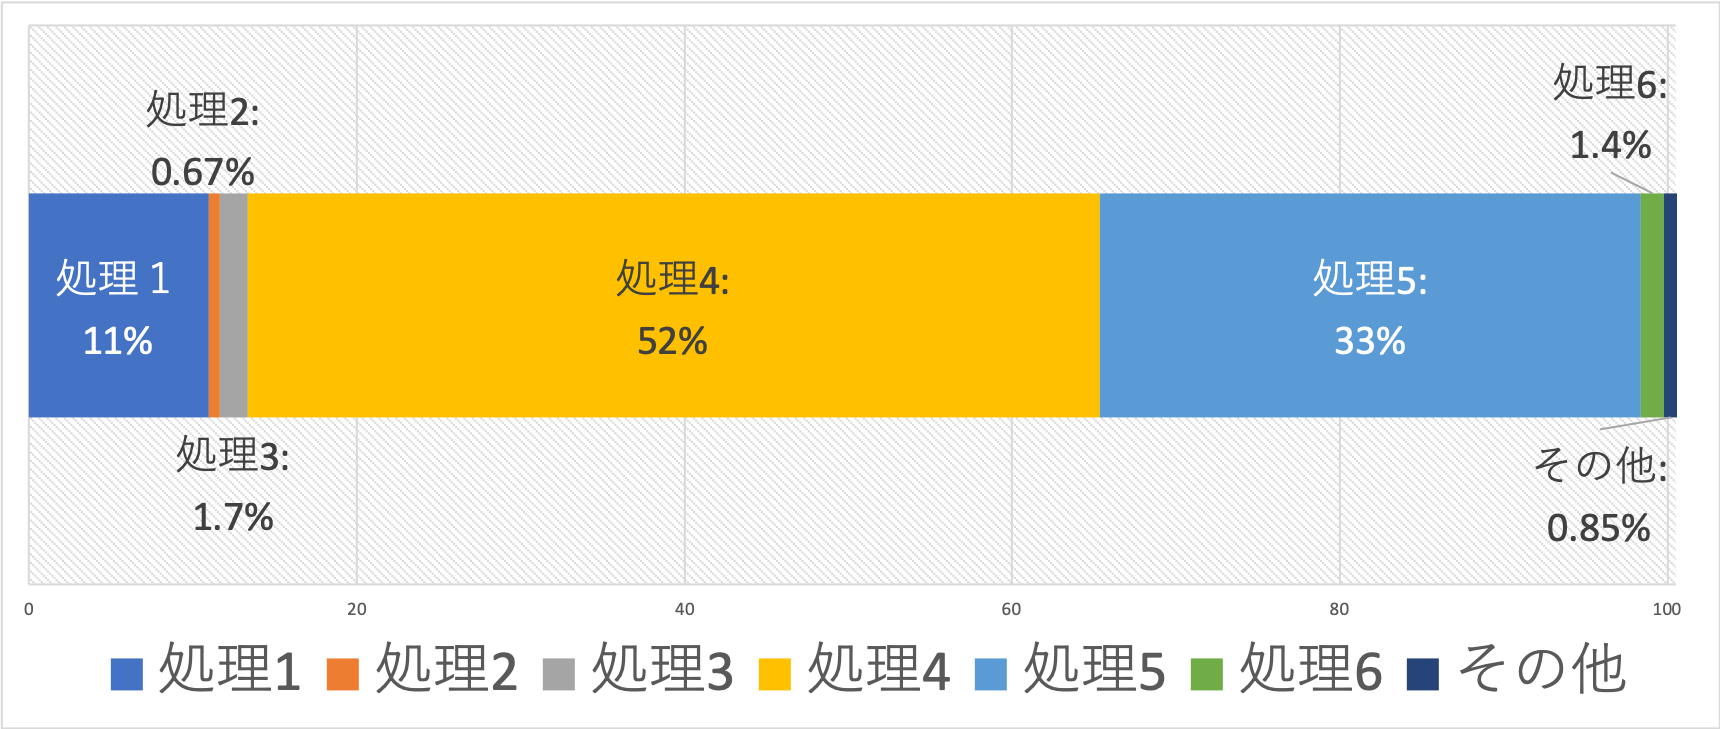
\includegraphics[width=8cm]{./upload_process_detail_gragh.png}
\end{center}
\end{minipage}
\begin{tablenotes}
\item[1] 1. 中央データベース接続、認証.
\item[2] 2. 中央データベース、ローカルデータベースからモジュール情報の取得.   
\item[3] 3. 中央データベースにFEチップ結果ページの作成。結果情報をアップロード. 
\item[4] 4. 2で作成した結果に対して、各データファイルを添付.  
\item[5] 5. 2で作成した結果に対して、各設定値ファイルを添付.   
\item[6] 6. 中央データベースにモジュールの結果ページの作成、結果情報をアップロード.  
\end{tablenotes}
\caption[アップロード機能における詳細処理測定結果]{アップロード機能における詳細処理測定結果。アップロード機能において、各詳細処理時間を測定した結果である。左図は測定値であり、右図はそれぞれの割合を示したものである。右図より、処理4、5の結果ファイルの添付、設定値ファイルの添付に多く時間がかかっていることが分かる。}
\label{upload_process_detail_result}
\end{figure}

\subsubsection{生産時における見積もり}
Quadモジュールにおける読み出し試験結果アップロード処理合計時間の見積もりを行った。
上述した測定はSCCであるためFEチップに対する処理は1回であるため、Quadモジュールの場合は表\ref{upload_process_detail_result}を用いて以下のように計算できる。
\bbb
{\rm FE}チップ処理&:& \left\{ (2.2+68+44) \pm \sqrt{(0.1)^2 + 3^2 + 0^2}  \right\}\times 4 \nonumber \\
&=& (4.6 \pm 0.1 ) \times 10^2 [{\rm sec}]\\\\
合計&:& (4.6 \pm 0.1 ) \times 10^2 [\rm{sec}]+ (14\pm0) + (0.88 \pm 0.14) + (1.8\pm0.1) \nonumber \\
&=& 7.9 \pm 0.1 [{\rm min}]
\eee

モジュール読み出し試験1回に対して、約8分程度かかる見積もりとなった。
円滑なモジュール組み立て、データ管理を行うために同期は速やかに行われることが要求されること、外観検査や平坦性測定のように他の品質試験も同期する必要があることを考慮し、処理時間の改善を試みた。
詳細を以下で示す。


\subsection{改善策}

図\ref{upload_process_detail_result}より処理4、5のファイル添付に大きく要していることが分かる。
この現状を踏まえ、各ファイルにおける添付処理時間の測定を行った。
測定は上述したものと同様にKEKサーバーを用いて合計20回行った。
添付する結果データファイル、設定ファイルの種類とデータ容量、添付処理実行結果、処理時間を表\ref{upload_status_to_pd}に示す。
ここで4MBを超える容量のファイル添付は失敗していることがわかり、アップロード機能の問題点を発見した。

{ \scriptsize
\begin{longtable}{|llllll|}
  \caption[アップロード処理における結果、設定値ファイル添付実行結果と処理時間]{アップロード処理における結果、設定値ファイル添付実行結果と処理時間。図\ref{upload_process_detail_result}より、読み出し試験に対して出力される各ファイルのアップロード実行結果、データ容量と処理時間をまとめた。ここで扱うファイルサイズの合計は94MBである。図よりファイルのデータ容量が大きいほど処理時間が長いことが分かる。std$\_$thresholdscanのようにファイル数が多い項目の場合、合計して大きい処理時間を要することが分かる。全項目において読み出しの設定ファイルにあたるbeforeCfg$\_$chipCfg.json、afterCfg$\_$chipCfg.jsonのアップロードは、中央データベースの容量制限により失敗していることが分かる。(texの技術的にcaptionが複数になってしまう。)}
  \label{upload_status_to_pd}
  \endhead
  \hline
  読み出し項目 & ファイル名 & 実行結果 & 容量[KB] & 処理時間[sec] & 全体[sec]\\ 
  \hline
std$\_$digitalscan & EnMask.json & Ok & 1,300 & 3.3 $\pm$ 0.1 & 17$\pm$0 \\
 & OccupancyMap.json & Ok & 1.500 & 2.9 $\pm$ 0.2 & \\
 & L1Dist.json & Ok & 0.53 & 0.75 $\pm$ 0.12 & \\
 & ctrlCfg$\_$ctrlCfg.json & Ok & 0.46 & 0.61 $\pm$ 0.08 & \\
 & dbCfg$\_$dbCfg.json & Ok & 0.60 & 0.69 $\pm$ 0.16 & \\
 & siteCfg$\_$siteCfg.json & Ok & 0.033 & 0.61 $\pm$ 0.06 & \\
 & userCfg$\_$userCfg.json & Ok & 0.14 & 0.66 $\pm$ 0.09 & \\
 & scanCfg$\_$std$\_$digitalscan.json & Ok & 2.2 & 0.55 $\pm$ 0.06 & \\
 & beforeCfg$\_$chipCfg.json & { \bf Error} & 7,200 & 3.0 $\pm$ 0.2 & \\
 & afterCfg$\_$chipCfg.json & { \bf Error} & 7,200 & 4.0 $\pm$ 0.2 & \\
\hline
std$\_$analogscan & EnMask.json & Ok & 1,300 & 3.9 $\pm$ 0.1 & 17$\pm$0\\
 & OccupancyMap.json & Ok & 1.400 & 2.6 $\pm$ 0.1 & \\
 & L1Dist.json & Ok & 0.60 & 0.69 $\pm$ 0.16 & \\
 & ctrlCfg$\_$ctrlCfg.json & Ok & 0.46 & 0.54 $\pm$ 0.05 & \\
 & dbCfg$\_$dbCfg.json & Ok & 0.60 & 0.49 $\pm$ 0.04 & \\
 & siteCfg$\_$siteCfg.json & Ok & 0.033 & 0.48 $\pm$ 0.04 & \\
 & userCfg$\_$userCfg.json & Ok & 0.14 & 0.58 $\pm$ 0.08 & \\
 & scanCfg$\_$std$\_$analogscan.json & Ok & 2.1 & 0.45 $\pm$ 0.03 & \\
 & beforeCfg$\_$chipCfg.json & { \bf Error} & 7,200 & 2.9 $\pm$ 0.2 & \\
 & afterCfg$\_$chipCfg.json & { \bf Error} & 7,200 & 3.9 $\pm$ 0.3 & \\
\hline
std$\_$thresholdscan & Scurve-30-96.json & Ok & 0.98 & 1.3 $\pm$ 0.1 & 49$\pm$1\\
 & Scurve-110-96.json & Ok & 0.98 & 0.45 $\pm$ 0.03 & \\
 & Scurve-70-96.json & Ok & 0.98 & 0.47 $\pm$ 0.04 & \\
 & Scurve-150-96.json & Ok & 1.0 & 0.46 $\pm$ 0.04 & \\
 & Scurve-190-96.json & Ok & 1.0 & 0.64 $\pm$ 0.12 & \\
 & Scurve-230-96.json & Ok & 1.0 & 0.49 $\pm$ 0.03 & \\
 & Scurve-270-96.json & Ok & 1.0 & 0.47 $\pm$ 0.04 & \\
 & Scurve-310-96.json & Ok & 1.0 & 0.47 $\pm$ 0.04 & \\
 & Scurve-350-96.json & Ok & 1.0 & 0.49 $\pm$ 0.03 & \\
 & Scurve-390-96.json & Ok & 1.0 & 0.52 $\pm$ 0.06 & \\
 & Scurve-40-96.json & Ok & 1.0 & 0.46 $\pm$ 0.03 & \\
 & Scurve-80-96.json & Ok & 0.99 & 0.68 $\pm$ 0.13 & \\
 & Scurve-120-96.json & Ok & 1.0 & 0.54 $\pm$ 0.07 & \\
 & Scurve-160-96.json & Ok & 1.0 & 0.51 $\pm$ 0.05 & \\
 & Scurve-200-96.json & Ok & 1.0 & 0.49 $\pm$ 0.04 & \\
 & Scurve-240-96.json & Ok & 1.0 & 0.50 $\pm$ 0.05 & \\
 & Scurve-280-96.json & Ok & 1.0 & 0.48 $\pm$ 0.04 & \\
 & Scurve-320-96.json & Ok & 1.0 & 0.49 $\pm$ 0.05 & \\
 & Scurve-360-96.json & Ok & 1.0 & 0.49 $\pm$ 0.06 & \\
 & Scurve-400-96.json & Ok & 1.0 & 0.45 $\pm$ 0.05 & \\
 & Scurve-10-96.json & Ok & 1.0 & 0.42 $\pm$ 0.03 & \\
 & Scurve-50-96.json & Ok & 0.99 & 0.49 $\pm$ 0.05 & \\
 & Scurve-90-96.json & Ok & 0.99 & 0.46 $\pm$ 0.05 & \\
 & Scurve-130-96.json & Ok & 1.0 & 0.47 $\pm$ 0.05 & \\
 & Scurve-170-96.json & Ok & 1.0 & 0.52 $\pm$ 0.04 & \\
 & Scurve-210-96.json & Ok & 1.0 & 0.51 $\pm$ 0.04 & \\
 & Scurve-250-96.json & Ok & 1.0 & 0.58 $\pm$ 0.10 & \\
 & Scurve-290-96.json & Ok & 1.0 & 0.64 $\pm$ 0.13 & \\
 & Scurve-330-96.json & Ok & 1.0 & 0.64 $\pm$ 0.09 & \\
 & Scurve-370-96.json & Ok & 1.0 & 0.49 $\pm$ 0.06 & \\
 & Scurve-60-96.json & Ok & 0.99 & 0.51 $\pm$ 0.06 & \\
 & Scurve-100-96.json & Ok & 1.0 & 0.48 $\pm$ 0.05 & \\
 & Scurve-140-96.json & Ok & 1.0 & 0.48 $\pm$ 0.06 & \\
 & Scurve-180-96.json & Ok & 1.0 & 0.52 $\pm$ 0.06 & \\
 & Scurve-220-96.json & Ok & 1.0 & 0.54 $\pm$ 0.05 & \\
 & Scurve-260-96.json & Ok & 1.0 & 0.51 $\pm$ 0.05 & \\
 & Scurve-300-96.json & Ok & 1.0 & 0.66 $\pm$ 0.09 & \\
 & Scurve-340-96.json & Ok & 1.0 & 0.51 $\pm$ 0.06 & \\
 & Scurve-380-96.json & Ok & 1.0 & 0.55 $\pm$ 0.05 & \\
 & sCurve-0.json & Ok & 49 & 1.0 $\pm$ 0.1 & \\
 & ThresholdDist-0.json & Ok & 4.6 & 0.56 $\pm$ 0.06 & \\
 & ThresholdMap-0.json & Ok & 2,200 & 4.3 $\pm$ 0.1 & \\
 & NoiseDist-0.json & Ok & 2.3 & 0.42 $\pm$ 0.04 & \\
 & Chi2Map-0.json & Ok & 2,300 & 4.5 $\pm$ 0.1 & \\
 & StatusMap-0.json & Ok & 1,300 & 2.8 $\pm$ 0.1 & \\
 & StatusDist-0.json & Ok & 0.49 & 0.48 $\pm$ 0.04 & \\
 & NoiseMap-0.json & Ok & 2,200 & 4.0 $\pm$ 0.2 & \\
 & Chi2Dist-0.json & Ok & 1.1 & 0.50 $\pm$ 0.04 & \\
 & TimePerFitDist-0.json & Ok & 3.1 & 0.56 $\pm$ 0.12 & \\
 & ctrlCfg$\_$ctrlCfg.json & Ok & 0.46 & 0.49 $\pm$ 0.05 & \\
 & dbCfg$\_$dbCfg.json & Ok & 0.60 & 0.52 $\pm$ 0.06 & \\
 & siteCfg$\_$siteCfg.json & Ok & 0.033 & 0.54 $\pm$ 0.07 & \\
 & userCfg$\_$userCfg.json & Ok & 0.14 & 0.60 $\pm$ 0.07 & \\
 & scanCfg$\_$std$\_$thresholdscan.json & Ok & 2.2 & 0.46 $\pm$ 0.03 & \\
 & beforeCfg$\_$chipCfg.json & { \bf Error} & 7,200 & 3.2 $\pm$ 0.2 & \\
 & afterCfg$\_$chipCfg.json & { \bf Error} & 7,200 & 3.5 $\pm$ 0.1 & \\
\hline
std$\_$totscan & MeanTotMap-0.json & Ok & 1,900 & 4.8 $\pm$ 0.1 & 20$\pm$0\\
 & SigmaTotMap-0.json & Ok & 2,200 & 4.1 $\pm$ 0.2 & \\
 & MeanTotDist-0.json & Ok & 0.59 & 0.54 $\pm$ 0.07 & \\
 & SigmaTotDist-0.json & Ok & 1.8 & 0.47 $\pm$ 0.03 & \\
 & L1Dist.json & Ok & 0.59 & 0.60 $\pm$ 0.08 & \\
 & ctrlCfg$\_$ctrlCfg.json & Ok & 0.46 & 0.47 $\pm$ 0.03 & \\
 & dbCfg$\_$dbCfg.json & Ok & 0.60 & 0.67 $\pm$ 0.24 & \\
 & siteCfg$\_$siteCfg.json & Ok & 0.033 & 0.59 $\pm$ 0.10 & \\
 & userCfg$\_$userCfg.json & Ok & 0.14 & 0.56 $\pm$ 0.05 & \\
 & scanCfg$\_$std$\_$totscan.json & Ok & 2.0 & 0.59 $\pm$ 0.10 & \\
 & beforeCfg$\_$chipCfg.json & { \bf Error} & 7,200 & 3.0 $\pm$ 0.1 & \\
 & afterCfg$\_$chipCfg.json & { \bf Error} & 7,200 & 3.9 $\pm$ 0.3 & \\
\hline
std$\_$noisescan & Occupancy.json & Ok & 1,300 & 4.0 $\pm$ 0.1 & 18$\pm$0\\
 & NoiseOccupancy.json & Ok & 1,300 & 2.5 $\pm$ 0.1 & \\
 & NoiseMask.json & Ok & 1,300 & 2.4 $\pm$ 0.1 & \\
 & ctrlCfg$\_$ctrlCfg.json & Ok & 0.46 & 0.57 $\pm$ 0.08 & \\
 & dbCfg$\_$dbCfg.json & Ok & 0.60 & 0.55 $\pm$ 0.06 & \\
 & siteCfg$\_$siteCfg.json & Ok & 0.033 & 0.53 $\pm$ 0.04 & \\
 & userCfg$\_$userCfg.json & Ok & 0.14 & 0.61 $\pm$ 0.07 & \\
 & scanCfg$\_$std$\_$noisescan.json & Ok & 1.4 & 0.53 $\pm$ 0.05 & \\
 & beforeCfg$\_$chipCfg.json & { \bf Error} & 7,200 & 2.8 $\pm$ 0.2 & \\
 & afterCfg$\_$chipCfg.json & { \bf Error} & 7,200 & 3.5 $\pm$ 0.1 & \\
\hline
\end{longtable}
}

\newpage
表\ref{upload_status_to_pd}より、データサイズの大きいものにアップロード時間がかかっていることがわかる。
また添付処理を行うオフセットがあることから、threshold scanのように各容量が大きくなくてもファイル数が多いものにはアップロード時間が合計して多くかかってしまうことがわかる。

これらのことと4MB以上の容量を持つファイル添付処理の失敗をなくすために、次のような改善策を考えた。

\begin{itemize}
  \item 各試験項目に対する結果データ、設定ファイルをそれぞれZipファイルに統合し、圧縮後にアップロードを行う。
\end{itemize}

こうすることで、アップロードするファイルの容量、数共に削減することができる。
圧縮率によってはアップロード処理の失敗もなくすことができると考えた。

これを踏まえアップロードツールを改良し、再び各ファイルの添付処理にかかる時間を測定した。
合計処理時間は以下のようになり、全てのファイルのアップロードに成功した。

\bbb
  36 \pm 1 [{\rm sec}]
\eee

{\scriptsize
\begin{longtable}{|llllll|}
  \caption[アップロード処理改善後における結果、設定値ファイル添付実行結果と処理時間]{アップロード処理改善後における結果、設定値ファイル添付実行結果と処理時間。各試験結果毎に結果ファイル、設定値ファイルをZipファイルにまとめアップロードする処理とした。これにより、ファイル数、容量の削減に成功し、アップロード時間が改善した。全てのファイルのアップロードに成功していることが分かる。}
  \label{upload_status_to_pd_zip}
  \endhead
  \hline
  読み出し項目 & ファイル名 & 実行結果 & 容量[KB] & 処理時間[sec] & 全体[sec] \\ 
  \hline
 std$\_$digitalscan & std$\_$digitalscan$\_$datafiles.zip & Ok & 10 & 0.77 $\pm$ 0.18 & 1.9 $\pm$ 0.2\\
 & std$\_$digitalscan$\_$configfiles.zip & Ok & 56 & 1.1 $\pm$ 0.1 &\\
\hline
 std$\_$analogscan & std$\_$analogscan$\_$datafiles.zip & Ok & 46 & 1.0 $\pm$ 0.2 & 2.2 $\pm$ 0.3 \\
 & std$\_$analogscan$\_$configfiles.zip & Ok & 58 & 1.2 $\pm$ 0.2 &\\
\hline
 std$\_$thresholdscan & std$\_$thresholdscan$\_$datafiles.zip & Ok & 1,500 & 2.6 $\pm$ 0.1 & 3.5 $\pm$ 0.1 \\
 & std$\_$thresholdscan$\_$configfiles.zip & Ok & 190 & 0.86 $\pm$ 0.08 &\\
\hline
 std$\_$totscan & std$\_$totscan$\_$datafiles.zip & Ok & 730 & 1.7 $\pm$ 0.2 & 2.5 $\pm$ 0.2\\
 & std$\_$totscan$\_$configfiles.zip & Ok & 190 & 0.83 $\pm$ 0.15 &\\
\hline
 std$\_$noisescan & std$\_$noisescan$\_$datafiles.zip & Ok & 19 & 0.56 $\pm$ 0.07 & 1.7 $\pm$ 0.1 \\
 & std$\_$noisescan$\_$configfiles.zip & Ok & 190 & 1.1 $\pm$ 0.1 &\\
\hline
\end{longtable}
}

\subsubsection{生産時における見積もり}
上記の見積もりと同様に、改善後のツールにおけるアップロード時間の見積もりを行った。
表\ref{upload_process_detail_result}において、添付処理に対応する処理4、5以外は同じとする。
改良後の処理4、5の処理時間は、
\bbb
{\rm FE}チップ処理&:& \left\{ (2.2+6.7+5.1) \pm \sqrt{(0.1)^2 + (1.1)^2 + (0.3)^2} \right\} \times 4 \\\nonumber 
&=& 56 \pm 5  [{\rm sec}] \\\\
合計&:& (56 \pm 5 )[\rm{sec}] + (14\pm0) + (0.88 \pm 0.14) + (1.8\pm0.1) \nonumber \\
&=& 1.2 \pm 0.1 [{\rm min}]
\eee

約1分でアップロードを完了できる見積もりとなった。
改善前に比べて15$\%$の処理時間となった。
現在は改善後の方法を用いたツールを提供している。

\clearpage
\subsubsection{ファイル添付以外の処理}
ここではファイル添付処理に関しての処理時間検討を行なったが、以下にあげたそれ以外の処理について言及する。
\begin{enumerate}
  \item ローカルデータベース内部処理.
  \item 中央データベースへの接続、認証処理.
  \item ファイル添付以外の処理に関して、中央データベースAPI使用.
  \item ネットワーク速度の改善.
\end{enumerate}

項目1に関して、読み出し試験におけるローカルデータベースの内部構造は世界的に使われているものである。
内部構造の変更をすることなく改善を図りたいという開発方針から、この項目に関しての処理時間削減の検討を行わなかった。
また図\ref{upload_process_detail_result}よりローカルデータベース内部処理は十分に小さいものであったため、検討の必要がないと考えた。

項目2に関して、中央データベースへの接続、認証処理は中央データベースのAPI及び中央データベースの内部構造によるものである。
この部分の処理を改善するには、これらの変更を検討する必要がある。

項目3に関して、アップロード処理では以下の処理の際に中央データベースのAPIを使用している。
\begin{itemize}
  \item モジュール情報の取得.
  \item 結果ページの作成(モジュールとFEチップで5回分)
\end{itemize}
これらの処理は必要であるため、APIの使用回数の減らし処理時間を削減することは難しい。

項目4に関して、中央データベースと通信する全ての処理はのネットワーク速度に依存していると考えられる(付録\ref{chap:data_time_detail})。
KEKのサーバーが置かれているネットワーク環境の改善により、本ツールの処理速度も改善すると考えられる。

